|\documentclass{article}
\usepackage[utf8]{inputenc}
\usepackage{graphicx}
\usepackage{adjustbox} % Potential solution?

\title{Camera based Water Stage and Discharge Prediction with Machine Learning}
\author{
Ernesto Adrián Álvarez Salazar  A00227490\\
Carlos Javier Leal Beltrán  A01741355\\
Carlos Moisés Chávez Jiménez  A01637322\\
Luis Armando Salazar López  A01114901\\
}
\date{Septiembre 2022 - Diciembre 2022}

\usepackage{listings}
\usepackage{color}

\definecolor{dkgreen}{rgb}{0,0.6,0}
\definecolor{gray}{rgb}{0.5,0.5,0.5}
\definecolor{mauve}{rgb}{0.58,0,0.82}

\lstset{frame=tb,
  language=Python,
  aboveskip=3mm,
  belowskip=3mm,
  showstringspaces=false,
  columns=flexible,
  basicstyle={\small\ttfamily},
  numbers=none,
  numberstyle=\tiny\color{gray},
  keywordstyle=\color{blue},
  commentstyle=\color{dkgreen},
  stringstyle=\color{mauve},
  breaklines=true,
  breakatwhitespace=true,
  tabsize=3
}

\begin{document}

\maketitle

\section{Introducción}

La medición y el modelado precisos del nivel (la altura del nivel del agua en el rio) y la descarga (el caudal del rio) de la corriente son importantes para la gestión diaria del agua, el pronóstico y la gestión de inundaciones, la evaluación del cumplimiento de los acuerdos de uso del agua y el diseño de embalses, sistemas de suministro de agua, puentes y alcantarillas (Boiten, 2008). Los datos continuos de series de tiempo de medidores de flujo también son críticos para calibrar y/o validar modelos de aguas superficiales y subterráneas, mientras que las brechas en estos datos aumentan la incertidumbre en las predicciones de un modelo.  El nivel de la corriente normalmente se mide con sensores flotantes, de presión, ópticos y acústicos (Turnipseed y Sauer, 2010).  Estos sensores tradicionales pueden fallar y requerir un mantenimiento regular, los cuales son costosos.  Como resultado, es posible que se produzcan lagunas en los registros de flujo y descarga debido a una instalación incorrecta (p. ej., especialmente durante estudios a corto plazo, cuando las características del sitio no son bien conocidas), fallas en los equipos y/o brechas en el financiamiento de los programas de monitoreo.  Por supuesto, las cámaras también pueden fallar, pero pueden proporcionar una redundancia económica con información que no está disponible en los sensores que emiten mediciones escalares individuales.  Por ejemplo, las imágenes proporcionan una verificación visual de las condiciones hidrológicas, incluida la presencia de hielo, obstrucciones o cambios importantes en la geometría del canal.  En este estudio, se opta por un enfoque al monitoreo pasivo que utiliza imágenes de lapso de tiempo que se pueden combinar con mediciones de sensores tradicionales que son adecuadas para llenar los vacíos en los registros de caudales.

\section{ Hipotesis}

Utilizando la investigación previamente realizada por el equipo del socio formador, mediante optimización de las imagenes utilizables en la problemática implementando librerias de computer vision en python, a través del desarrollo de modelos matemáticos y  el análisis de datos, se espera obtener formas distintas y optimizadas de abordar la problemática, modelos de regresión que nos permitan predecir el nivel y la descarga de una corriente con más eficacia y un modelo de clasificación que permita distinguir y optimizar entre imágenes utilizables dentro del proceso de obtención de datos, mejorando así en un aspecto general, la parte práctica en la resolución de esta problemática. 

\section{Tratamiento Inicial de los Datos}

Para comenzar a trabajar con los datos, es necesario que pasen por un proceso de preparación que nos permita obtener la mejor parte de ellos. Este proceso se divide en tres etapas: Limpieza, Transformación y Visualización. A continuación desglosaremos las fases involucradas a este proceso:

    \subsection{Limpieza de los datos}

        La limpieza es la primera y una etapa fundamental del tratamiento de la información. Aquí se busca eliminar la mayor cantidad de imperfecciones que pudieramos llegar a encontrar. Cosas como valores faltantes, datos fuera de rango, dividir la información disponible en "entrenamiento" y "pruebas", eliminar columnas innecesarias para el análisis, etc.\\

        \begin{adjustbox}{left=-0.25cm}

	\begin{tabular}{ |c | c| c| c |} 
        \hline
            SensorTime  & CaptureTime  & Filename  &  hlineAgency \\ 
             \hline
            SiteNumber  & TimeZone  & Stage  & Discharge \\
             \hline
            CalcTimestamp & fNumber  & isoSpeed  & shutterSpeed   \\
             \hline
            grayMean  & graySigma  & entropyMean  & entropySigma  \\
             \hline
            hMean  & hSigma  & sMean  & sSigma  \\
             \hline
            vMean  & vSigma  & areaFeatCount  & grayMean 0 \\
             \hline
            graySigma 0  &  entropyMean 0  &  entropySigma 0  &   hMean 0  \\
             \hline
            hSigma 0  &  sMean 0  &  sSigma 0  &  vMean 0  \\
             \hline
            vSigma 0  &  grayMean 0  &  graySigma 0  & entropyMean 0 \\
             \hline
            entropySigma 0  &  hMean 0  &  hSigma 0  & sMean 0 \\
             \hline
            sSigma 0  & vMean 0  &  vSigma 0  & WeirAngle  \\
             \hline
            WeirPt1X  & WeirPt1Y  & WeirPt2X  &  WeirPt2Y \\
             \hline
            WwRawLineMin  & WwRawLineMax  & WwRawLineMean  &  WwRawLineSigma \\
             \hline
            WwCurveLineMin  & WwCurveLineMax  &  WwCurveLineMean  & WwCurveLineSigma   \\
        \hline
        \end{tabular}
        \end{adjustbox}

       \begin{center}
           \textbf{Variables disponibles en nuestro archivo de datos. (figura 3.1.1)} \\
       \end{center}     
        

    \subsection{Transformación de los datos}
        Una vez revisados los datos, entendemos que debemos transformarlos para generar gráficos y diagramas que faciliten la búsqueda de patrones y la determinación de los parametros necesarios para un modelo predictor de regresión y uno de clasificación.
        
        Para esto, revisamos el conjunto de datos con la información proporcionada. Encontramos que primero debemos ordenar los datos con base en el timestamp. Esta variables que indican el tiempo con el que fueron realizadas las capturas de datos. Dentro del conjunto de datos se proporcionan tres variables para indicar el tiempo de captura: "CaptureTime","SensorTime" y "CalcTimestamp", y cada una de estas contiene un formato distinto y a primera instancia nada fácil de trabajar, lo que indica que tenemos que separarlas para que queden enumeradas de una en una. Desarrollamos un método para tratar las fechas consiguiendo así, un orden en el formato de la captura de datos. En cuanto a lo demás, los datos venían en buenas condiciones, por lo que no tuvimos que arreglar valores nulos. \\

    \subsection{Visualización de los datos}\\

        Siendo las variables "Stage" y "Discharge" las que nos iteresan predecir con un modelo, las comparamos con el resto de las variables para ir descartando las de menor correlacion.

        \begin{center}
            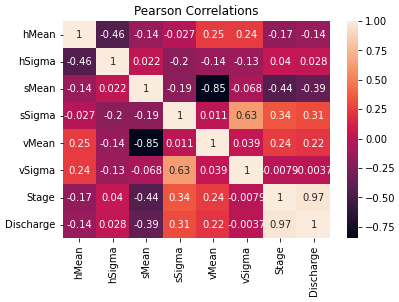
\includegraphics{images/Corr_pearson4.PNG} \\
            
           \textbf{Ejemplo de las correlaciones de pearson realizadas. (figura 3.3.1 )} \\


       \end{center}   


        Tras comparar con y analizar cada una de las variables dentro del conjunto de datos con las variables stage y discharge escogimos las siguientes variables, ya que cuentan con una correlación menor a -30 ó mayor a 30, por lo tanto tienen una correlación considerable para incluirse en un modelo: sSigma, grayMean 0, hMean 0, grayMean 1, hMean 1, sMean s, Sigma 1, WeirPt1Y, WeirPt2X, WeirPt2Y. 




    \section{Generación y evaluación de los modelos de predicción para Discharge y Stage.}
    Tras identificar las variables que deseamos predecir y las variables que podemos utilizar para lograrlo, comenzamos a realizar modelos con el fin de obtener resultados similares a la investigación pasada, lo anterior con el fin de contar con un punto de partida. \\

    Con la finalidad de mantener nuestros datos más limpios y prevenir que los modelos implementados caigan en un "overfitting" separamos nuestros datos en tres categorías: "Training" cuyo proposito es entrenar al modelo, "Testing" cuyo proposito es probar que tan bien entrenado se encuentra el modelo conforme a los datos del training y por último "Validation" cuyo proposito es presentar imagenes nuevas que validen el modelo una vez probado, con la finalidad de comprobar que el modelo reacciona bien ante datos nuevos. 

    

    \subsection{Stage}\\

    Inicialmente generamos un modelo regresor con Random Forest sin limpiar los datos para comprobar la fiabilidad mostrada en la investigacipon inicial. Los resultados obtenidos fueron los siguientes:\\
    \\
    {R^{2}}:  0.8337732202287705 \\
    MSE:  0.10366011037446508 \\
    RSMSE:  0.32196290217114315\\
    MAE:  0.1533417855444603\\
    Error estandar:  0.3219642351177667\\

        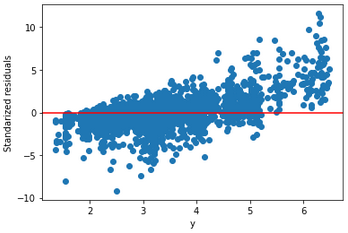
\includegraphics[scale=0.5]{images/residuos-stage-randomforest1.PNG} 
        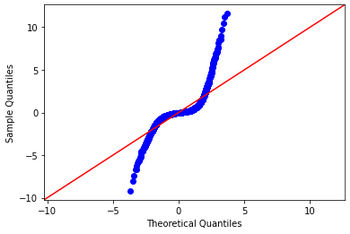
\includegraphics[scale=0.5]{images/residuos-stage-quantil1.PNG} \\
        \begin{center}
            \textbf{Gráfico de residuos y cuantíl. (figuras 4.1.1 y 4.1.2)}
        \end{center}
        

Utilizaremos también los modelos Multi Layer Perceptron y Support Vector Regression para contrastarlos con los del paper.\\
Resultados del MLP:\\
    \\
    {R^2}:  0.8452408041827444\\
    MSE:  0.09650884978917687\\
    RSMSE:  0.31065873525329507\\
    MAE:  0.153458677001836\\
    Error estandar:  0.31070539268642416\\

        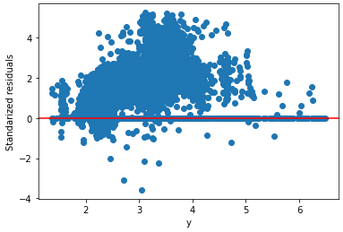
\includegraphics[scale=0.6]{residuos-stage-MLP1.PNG} 
        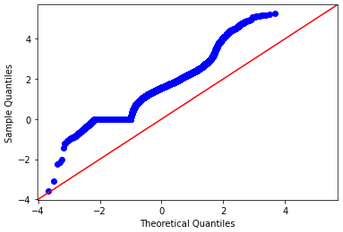
\includegraphics[scale=0.6]{residuos-stage-quantil2.PNG} \\
        \begin{center}
            \textbf{Gráfico de residuos y cuantíl. (figuras 4.1.3 y 4.1.4)}
        \end{center}


    Resultados del SVR:\\
    \\
    {R^2}:  0.8068711443896812\\
    MSE:  0.12043642135528387\\
    RSMSE:  0.34703950979000053\\
    MAE:  0.18047332110724765\\
    Error estandar:  0.3467160676989866\\


        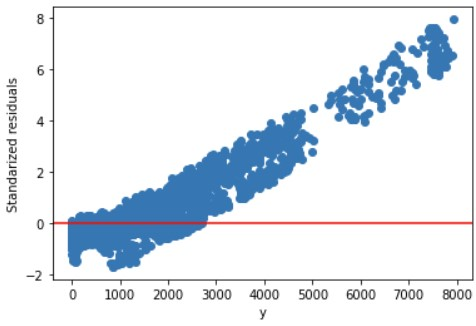
\includegraphics[scale=0.6]{residuos-stage-SVR1.PNG} 
        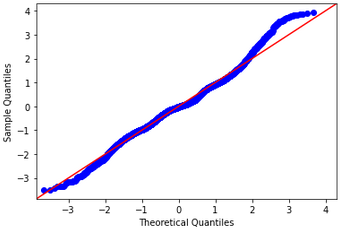
\includegraphics[scale=0.6]{residuos-stage-quantil3.PNG} \\
        \begin{center}
            \textbf{Gráfico de residuos y cuantíl. (figuras 4.1.5 y 4.1.6)}
        \end{center}


Generaremos ahora un modelo regresión de tipo mínimos cuadrados ordinarios. Esto nos permitirá comparar este modelo con el anterior de Random Forest.\\

Resultados del OLS:\\
{R^{2}}:  0.5771135725862011\\
MSE:  0.26371475042654247\\
RSMSE:  0.5135316450098694\\
MAE:  0.34110993914908105\\
Error estandar:  0.5133338519175923\\


        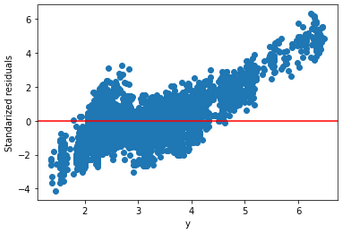
\includegraphics[scale=0.6]{residuos-stage-OLS1.PNG} 
        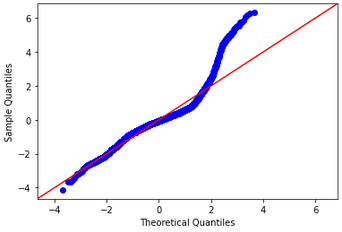
\includegraphics[scale=0.6]{residuos-stage-quantil4.PNG} \\
        \begin{center}
            \textbf{Gráfico de residuos y cuantíl. (figuras 4.1.7 y 4.1.8)}\\
        \end{center}

\subsection{Lasso y  factor de inflación de varianza}

Utilizaremos dos metodos para conocer saber si las variables independientes que elegimos tienen la suficiente influencia para quedarse en el modelo.\\

El primero será Lasso. Este método nos otorga los coeficientes de cada variable para ver cuál tiene más influencia que otras.\\

Los resultados obtenidos fueron los siguientes:\\

\begin{center}
        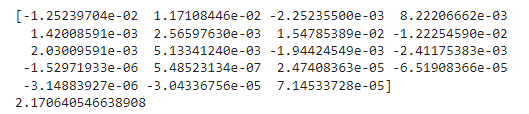
\includegraphics[scale=0.7]{stage-lasso.PNG} \\
        \textbf{Coeficientes obtenidos mediante LASSO. (figura 4.2.1)}
\end{center}

El segundo método es con el factor de inflación de varianza. Este también nos muestra la influencia que tiene cada variable con la que queremos proyectar. En dado caso que una salga con un factor de inflación de varianza de más de 10, qué en general, un VIF superior a 10 indica una alta correlación y es motivo de preocupación, la descataremos por tener una relación directa de la variable a proyectar. Lo cual generaría una desviación del modelo.\\

Los resultados obtenidos fueron los siguientes:\\

\begin{center}
        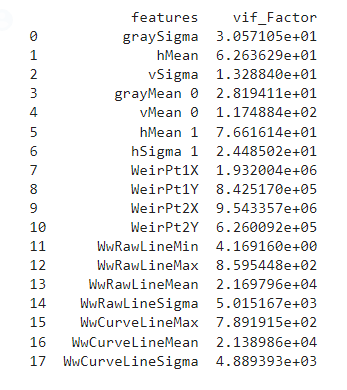
\includegraphics[scale=0.7]{stage-variance-inflation.PNG} \\
        \textbf{VIFs obtenidos. (figura 4.2.2)}
\end{center}

Obtuvimos valores atípicos conforme a los siguientes métodos:

            \begin{itemize}
                \item Valores atípicos de residuos
                \item Valores altos de apalancamiento
                \item Valores altos de distancia de Cook
                \item Valores altos de DFFIT
                \item  Valores altos de DFBetas 
            \end{itemize}
   

|Una vez que obtuvimos estos valores, los eliminamos de nuestros datos de entrenamiento con el fin de ver si logramos generar mejores modelos. Habiendo eliminado los valores atípicos, generaremos los mismo modelos para ver si obtenemos una mejor efectividad.\\

|Empezaremos generando primero un modelo con Random Forest por ser el que se utilizó en el Paper. Verémos si podemos generar una efectividad mayor a la mencionada por los investigadores.\\

Resultados del Random Forest trás eliminar datos atípicos
:\\
    \\
    {R^2}:  0.8272486821654673\\
    MSE:  0.1077288551141227\\
    RSMSE:  0.3282207414441121\\
    MAE:  0.15628777936281502\\
    Error estandar:  0.32824741648132333\\
    
        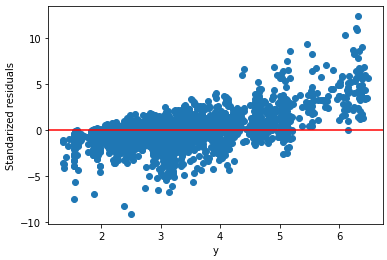
\includegraphics[scale=0.6]{residuos-stage-randomforest2.PNG} 
        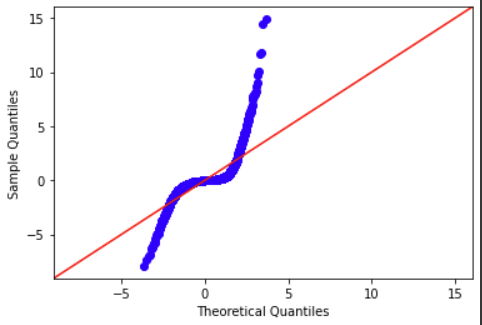
\includegraphics[scale=0.6]{residuos-stage-RFR-quantil.PNG} \\
        \begin{center}
            \textbf{Gráfico de residuos y cuantíl. (figuras 4.2.3 y 4.2.4)}
        \end{center}

Ahora, generaremos uno con MLP. Esto para contrastar su efectividad con la de Random Forest y comparar cuál es mejor.\\

Resultados del MLP trás eliminar datos atípicos
:\\

        {R^2}:  0.8366963392403801\\
        MSE:  0.10183723418208397\\
        RSMSE:  0.3191194669431559\\
        MAE:  0.1608734256261398\\
        Error estandar:  0.31601780927805584\\

        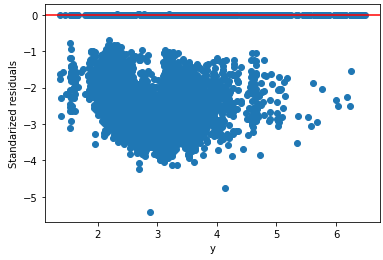
\includegraphics[scale=0.6]{residuos-stage-MLP-2.PNG} 
        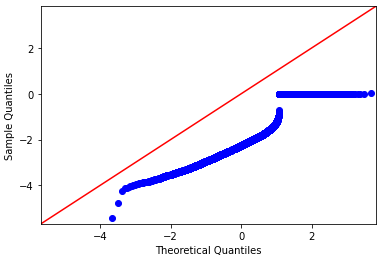
\includegraphics[scale=0.6]{residuos-stage-MLP-quantil.PNG} \\
                \begin{center}
            \textbf{Gráfico de residuos y cuantíl. (figuras 4.2.5 y 4.2.6)}
        \end{center}


Lo mismo con SVR:\\

        {R^2}:  0.8068711443896812\\
        MSE:  0.12043642135528387\\
        RSMSE:  0.34703950979000053\\
        MAE:  0.18047332110724765\\
        Error estandar:  0.3467160676989866\\


        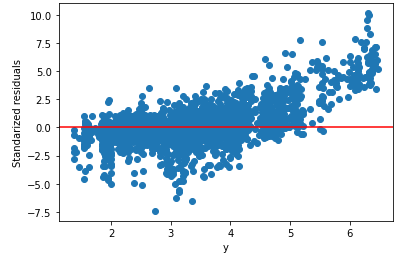
\includegraphics[scale=0.6]{residuos-stage-SVR-2.PNG} 
        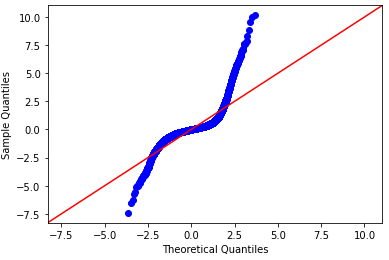
\includegraphics[scale=0.6]{residuos-stage-SVR-quantil.PNG} \\
                \begin{center}
            \textbf{Gráfico de residuos y cuantíl. (figuras 4.2.7 y 4.2.8)}
        \end{center}

Podemos comparar los resultados antes y después de retirar residuos observando la figura 4.2.9, en la cual indicamos el método y el método sin residuos con la expresión "s/r":\\

\begin{tabular}{|c|c|c|c|c|c|}
    \hline
    Method  &   R-squared  & MSE & RSMSE & MAE & Std Error  \\
    \hline
    RFR & 0.83377 & 0.10366 & 0.32196 & 0.15334 &  0.32196\\
    \hline
    RFR - s/r  & 0.82724 & 0.10772 & 0.32822 & 0.15628 &  0.32824\\
    \hline
    MLP & 0.84524 & 0.09650 & 0.31065 & 0.15345 & 0.31070 \\
    \hline
    MLP - s/r & 0.83669 & 0.10183 & 0.31911 & 0.16087 & 0.31601 \\
    \hline
    SVR & 0.80687 & 0.12043 & 0.34703 & 0.18047 & 0.34671 \\
    \hline
    SVR - s/r & 0.80687 & 0.12043 & 0.34703 & 0.18047 & 0.34671 \\
    \hline
    OLS & 0.57711 & 0.26371 & 0.51353 & 0.34110 & 0.51333 \\
    \hline
\end{tabular}

\begin{center}
            \textbf{Tabla de comparación de métricas. (figura 4.2.9)}
\end{center}



\subsection{Discharge}

    Inicialmente generamos un modelo regresor con Random Forest sin limpiar los datos para comprobar la fiabilidad mostrada en la investigacipon inicial. Los resultados obtenidos fueron los siguientes:\\
    \\
    {R^2}:  0.8247287083095377\\
    MSE:  233956.12149014932\\
    RSMSE:  483.690108943887\\
    MAE:  200.22409922729435\\
    Error estandar:  483.5868563381082\\


        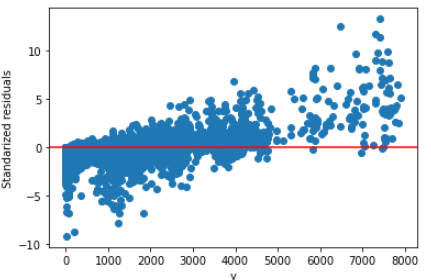
\includegraphics[scale=0.6]{residuos-discharge-randomforest1.PNG}
        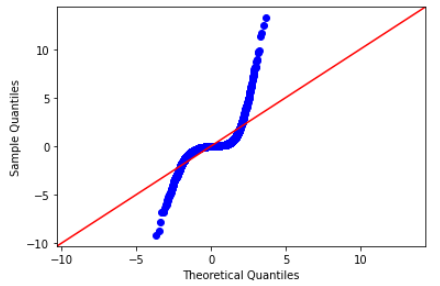
\includegraphics[scale=0.6]{residuos-discharge-quantil1.PNG} \\
                \begin{center}
            \textbf{Gráfico de residuos y cuantíl. (figuras 4.3.1 y 4.3.2)}
        \end{center}



    |Utilizaremos también los modelos MLP y SVR para contrastarlos con los del paper.\\
Resultados del MLP:\\
    {R^2}:  0.9106606310053236\\
    MSE:  119252.22929996347\\
    RSMSE:  345.3291608016379\\
    MAE:  157.9595011798805\\
    Error estandar:  345.3897105087386\\
                                                         



        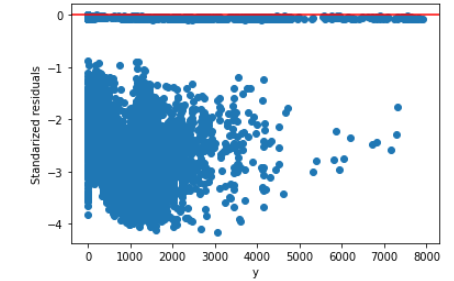
\includegraphics[scale=0.6]{residuos-discharge-MLP1.PNG} 
        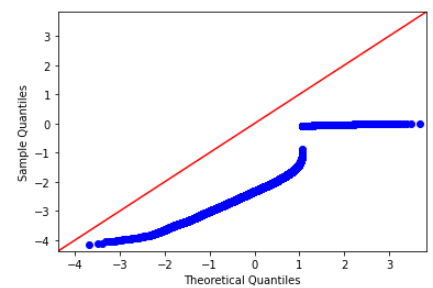
\includegraphics[scale=0.6]{residuos-discharge-quantil2.PNG} \\
        \begin{center}
            \textbf{Gráfico de residuos y cuantíl. (figuras 4.3.3 y 4.3.4)}
        \end{center}


    Resultados del SVR:\\
    {R^2}:  0.47833182204956115\\
    MSE:  696334.5933095505\\
    RSMSE:  834.4666520056692\\
    MAE:  370.20593703858617\\
    Error estandar:  818.5175314021255\\

    Los gráficos de residuos y cuantíl lucen así: 

        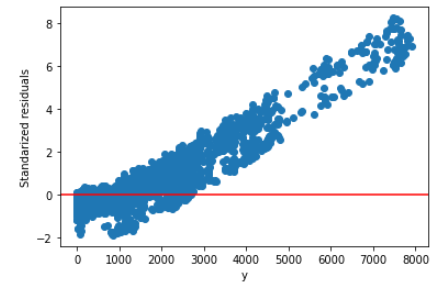
\includegraphics[scale=0.6]{residuos-discharge-SVR1.PNG} 
        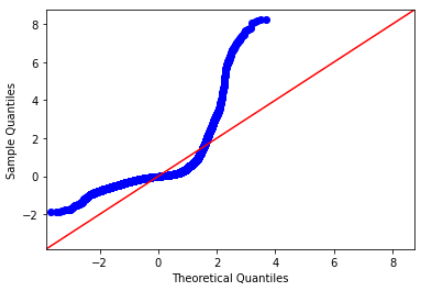
\includegraphics[scale=0.6]{residuos-discharge-quantil3.PNG} \\
        \begin{center}
            \textbf{Gráfico de residuos y cuantíl. (figuras 4.3.5 y 4.3.6)}
        \end{center}        


Generaremos ahora un modelo regresión de tipo mínimos cuadrados ordinarios. Esto nos permitirá comparar este modelo con el anterior de Random Forest.\\

Resultados del OLS:\\
{R^2}:  0.5825741299373127\\
MSE:  557189.5809496772\\
RSMSE:  746.4513252380741\\
MAE:  471.07220350721855\\
Error estandar:  746.029710625578\\


    Los gráficos de residuos y cuantíl lucen así: 

        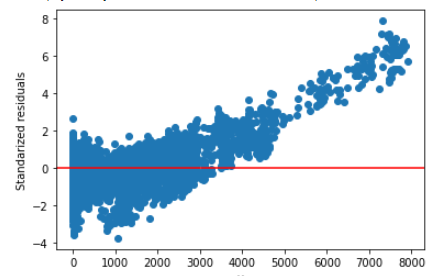
\includegraphics[scale=0.6]{residuos-discharge-OLS1.PNG} 
        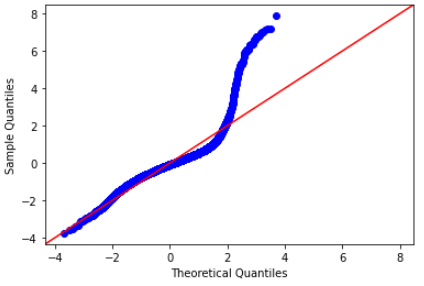
\includegraphics[scale=0.6]{residuos-discharge-quantil4.PNG} \\
        \begin{center}
            \textbf{Gráfico de residuos y cuantíl. (figuras 4.3.7 y 4.3.8)}
        \end{center}


 
\subsection{Lasso y  factor de inflación de varianza}\\

Una vez más, utilizaremos LASSO y VIF para conocer saber si las variables independientes que elegimos tienen la suficiente influencia para quedarse en el modelo.\\

Los resultados obtenidos fueron los siguientes:\\

\begin{center}
        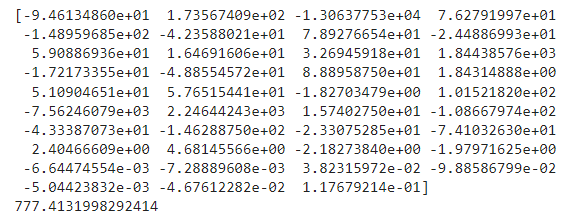
\includegraphics[scale=0.5]{images/lasso-discharge-1.PNG} \\
        \textbf{Coeficientes obtenidos mediante LASSO. (figura 4.4.1)}
        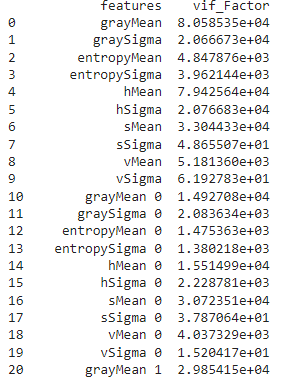
\includegraphics[scale=0.5]{discharge-variance-inflation-1.PNG} 
        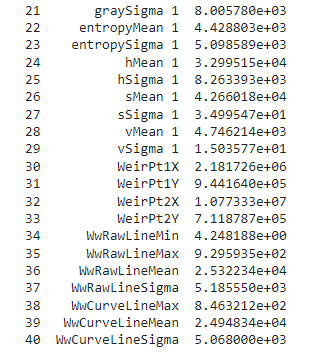
\includegraphics[scale=0.5]{discharge-variance-inflation-2.PNG} \\
        \textbf{VIFs obtenidos. (figura 4.4.2)}\\
        
\end{center}        



|Una vez que obtuvimos estos valores, los eliminamos de nuestros datos de entrenamiento con el fin de ver si logramos generar mejores modelos. Habiendo eliminado los valores atípicos, generaremos los mismo modelos para ver si obtenemos una mejor efectividad.\\

|Empezaremos generando primero un modelo con Random Forest por ser el que se utilizó en el Paper. Verémos si podemos generar una efectividad mayor a la mencionada por los investigadores.\\

Resultados del Random Forest trás eliminar datos atípicos
:\\
    \\
        $R^2:  0.823540678021367\\
        MSE:  235541.9314408406\\
        RSMSE:  485.32662346180905\\
        MAE:  200.50039029957205\\
        Error estandar:  485.2362009818441\\

        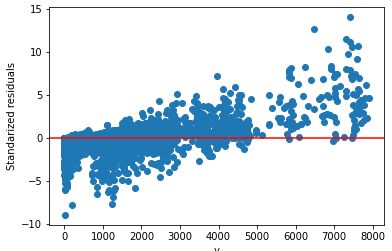
\includegraphics[scale=0.6]{residuos-discharge-randomforest2.PNG} 
        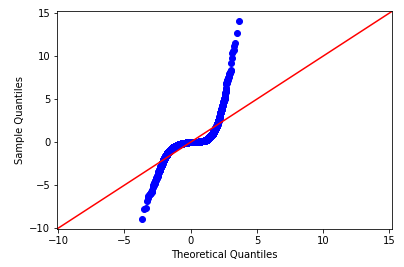
\includegraphics[scale=0.6]{residuos-discharge-RFR-quantil.PNG} \\
        \begin{center}
            \textbf{Gráfico de residuos y cuantíl. (figuras 4.4.3 y 4.4.4)}
        \end{center}
        \\
        

Ahora, generaremos uno con MLP. Esto para contrastar su efectividad con la de Random Forest y comparar cuál es mejor.\\

Resultados del MLP trás eliminar datos atípicos
:\\
        
        $R^2:  0.9059160163932675\\
        MSE:  125585.44920092999\\
        RSMSE:  354.38037361136406\\
        MAE:  165.7657409533583\\
        Error estandar:  354.0705546392842\\



        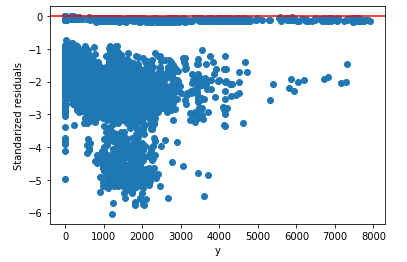
\includegraphics[scale=0.6]{residuos-discharge-MLP-2.PNG} 
        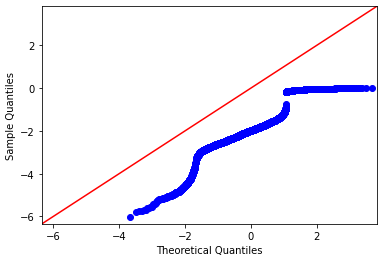
\includegraphics[scale=0.6]{residuos-discharge-MLP-quantil.PNG} \\
        \begin{center}
            \textbf{Gráfico de residuos y cuantíl. (figuras 4.4.5 y 4.4.6)}
        \end{center}
        

Lo mismo con SVR:\\

        {R^2}:  0.47833182204956115\\
        MSE:  696334.5933095505\\
        RSMSE:  834.4666520056692\\
        MAE:  370.20593703858617\\
        Error estandar:  818.5175314021255\\


        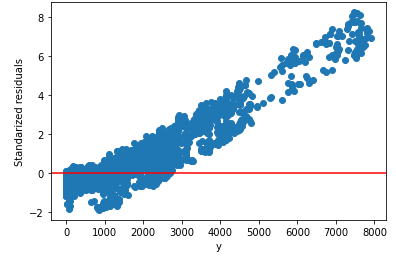
\includegraphics[scale=0.6]{residuos-discharge-SVR-2.PNG} 
        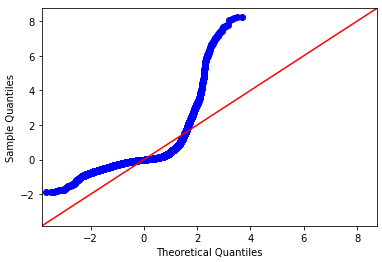
\includegraphics[scale=0.6]{residuos-discharge-SVR-quantil.PNG}
        \begin{center}
            \textbf{Gráfico de residuos y cuantíl. (figuras 4.4.7 y 4.4.8)}
        \end{center}

Podemos comparar los resultados antes y después de retirar residuos observando la figura 4.2.9, en la cual indicamos el método y el método sin residuos con la expresión "s/r":\\

\begin{tabular}{|c|c|c|c|c|c|}
    \hline
    Method  &   R-squared  & MSE & RSMSE & MAE & Std Error  \\
    \hline
    RFR & 0.82472 & 233956.1214 & 483.6901 & 200.2240 &   483.5868\\
    \hline
    RFR - s/r  & 0.82354 & 235541.9314 & 485.3266 & 200.5003 &  485.2362\\
    \hline
    MLP & 0.91066 & 119252.2292 & 345.3291 & 157.9595 & 345.3897 \\
    \hline
    MLP - s/r & 0.90591 & 25585.4492 & 354.3803 & 165.7657 & 354.0705 \\
    \hline
    SVR & 0.47833 & 696334.5933 & 834.4666 & 370.2059 & 818.5175 \\
    \hline
    SVR - s/r & 0.47833 & 696334.5933 & 834.4666 & 370.2059 & 818.5175 \\
    \hline
    OLS & 0.58257 & 557189.5809 & 746.4513 & 471.0722 & 746.0297 \\
    \hline

\end{tabular}

\begin{center}
            \textbf{Tabla de comparación de métricas. (figura 4.4.9)}
\end{center}

\subsection{Acercamiento}

Trás analizar las figuras 4.2.9, 4.4.9 y observar con detalle nuestros resultados llegamos a dos puntos de interés:\\

Es más sencillo predecir el discharge de un cuerpo de agua que su stage, esto es una observación de utilidad para investigaciones futúras.\\
    
Si bien tenemos modelos que logran predecir de manera convincente tanto stage como discharge, el aporte que deseamos proveer con nuestro trabajo a la investigación previa tiene como intención no solo proveer modelos alternativos para la predicción sino también optimizar el proceso de entrenamiento e introducción de imágenes válidas a redes comvolucionales. 


\section{Deep Learning aplicado a la problemática}

Con la finalidad de realizar análisis óptimo de la alta cantidad de imagenes proporcionadas por el socio formador, como equipo optamos por un modelo de clasificación binario aplicado a las imagenes,el modelo tiene como proposito principal, separar las imágenes optimas para análisis, de las imágenes con altas cantidades de ruido, ya sea obscuras, congeladas o inundadas.\\  
\begin{center}
        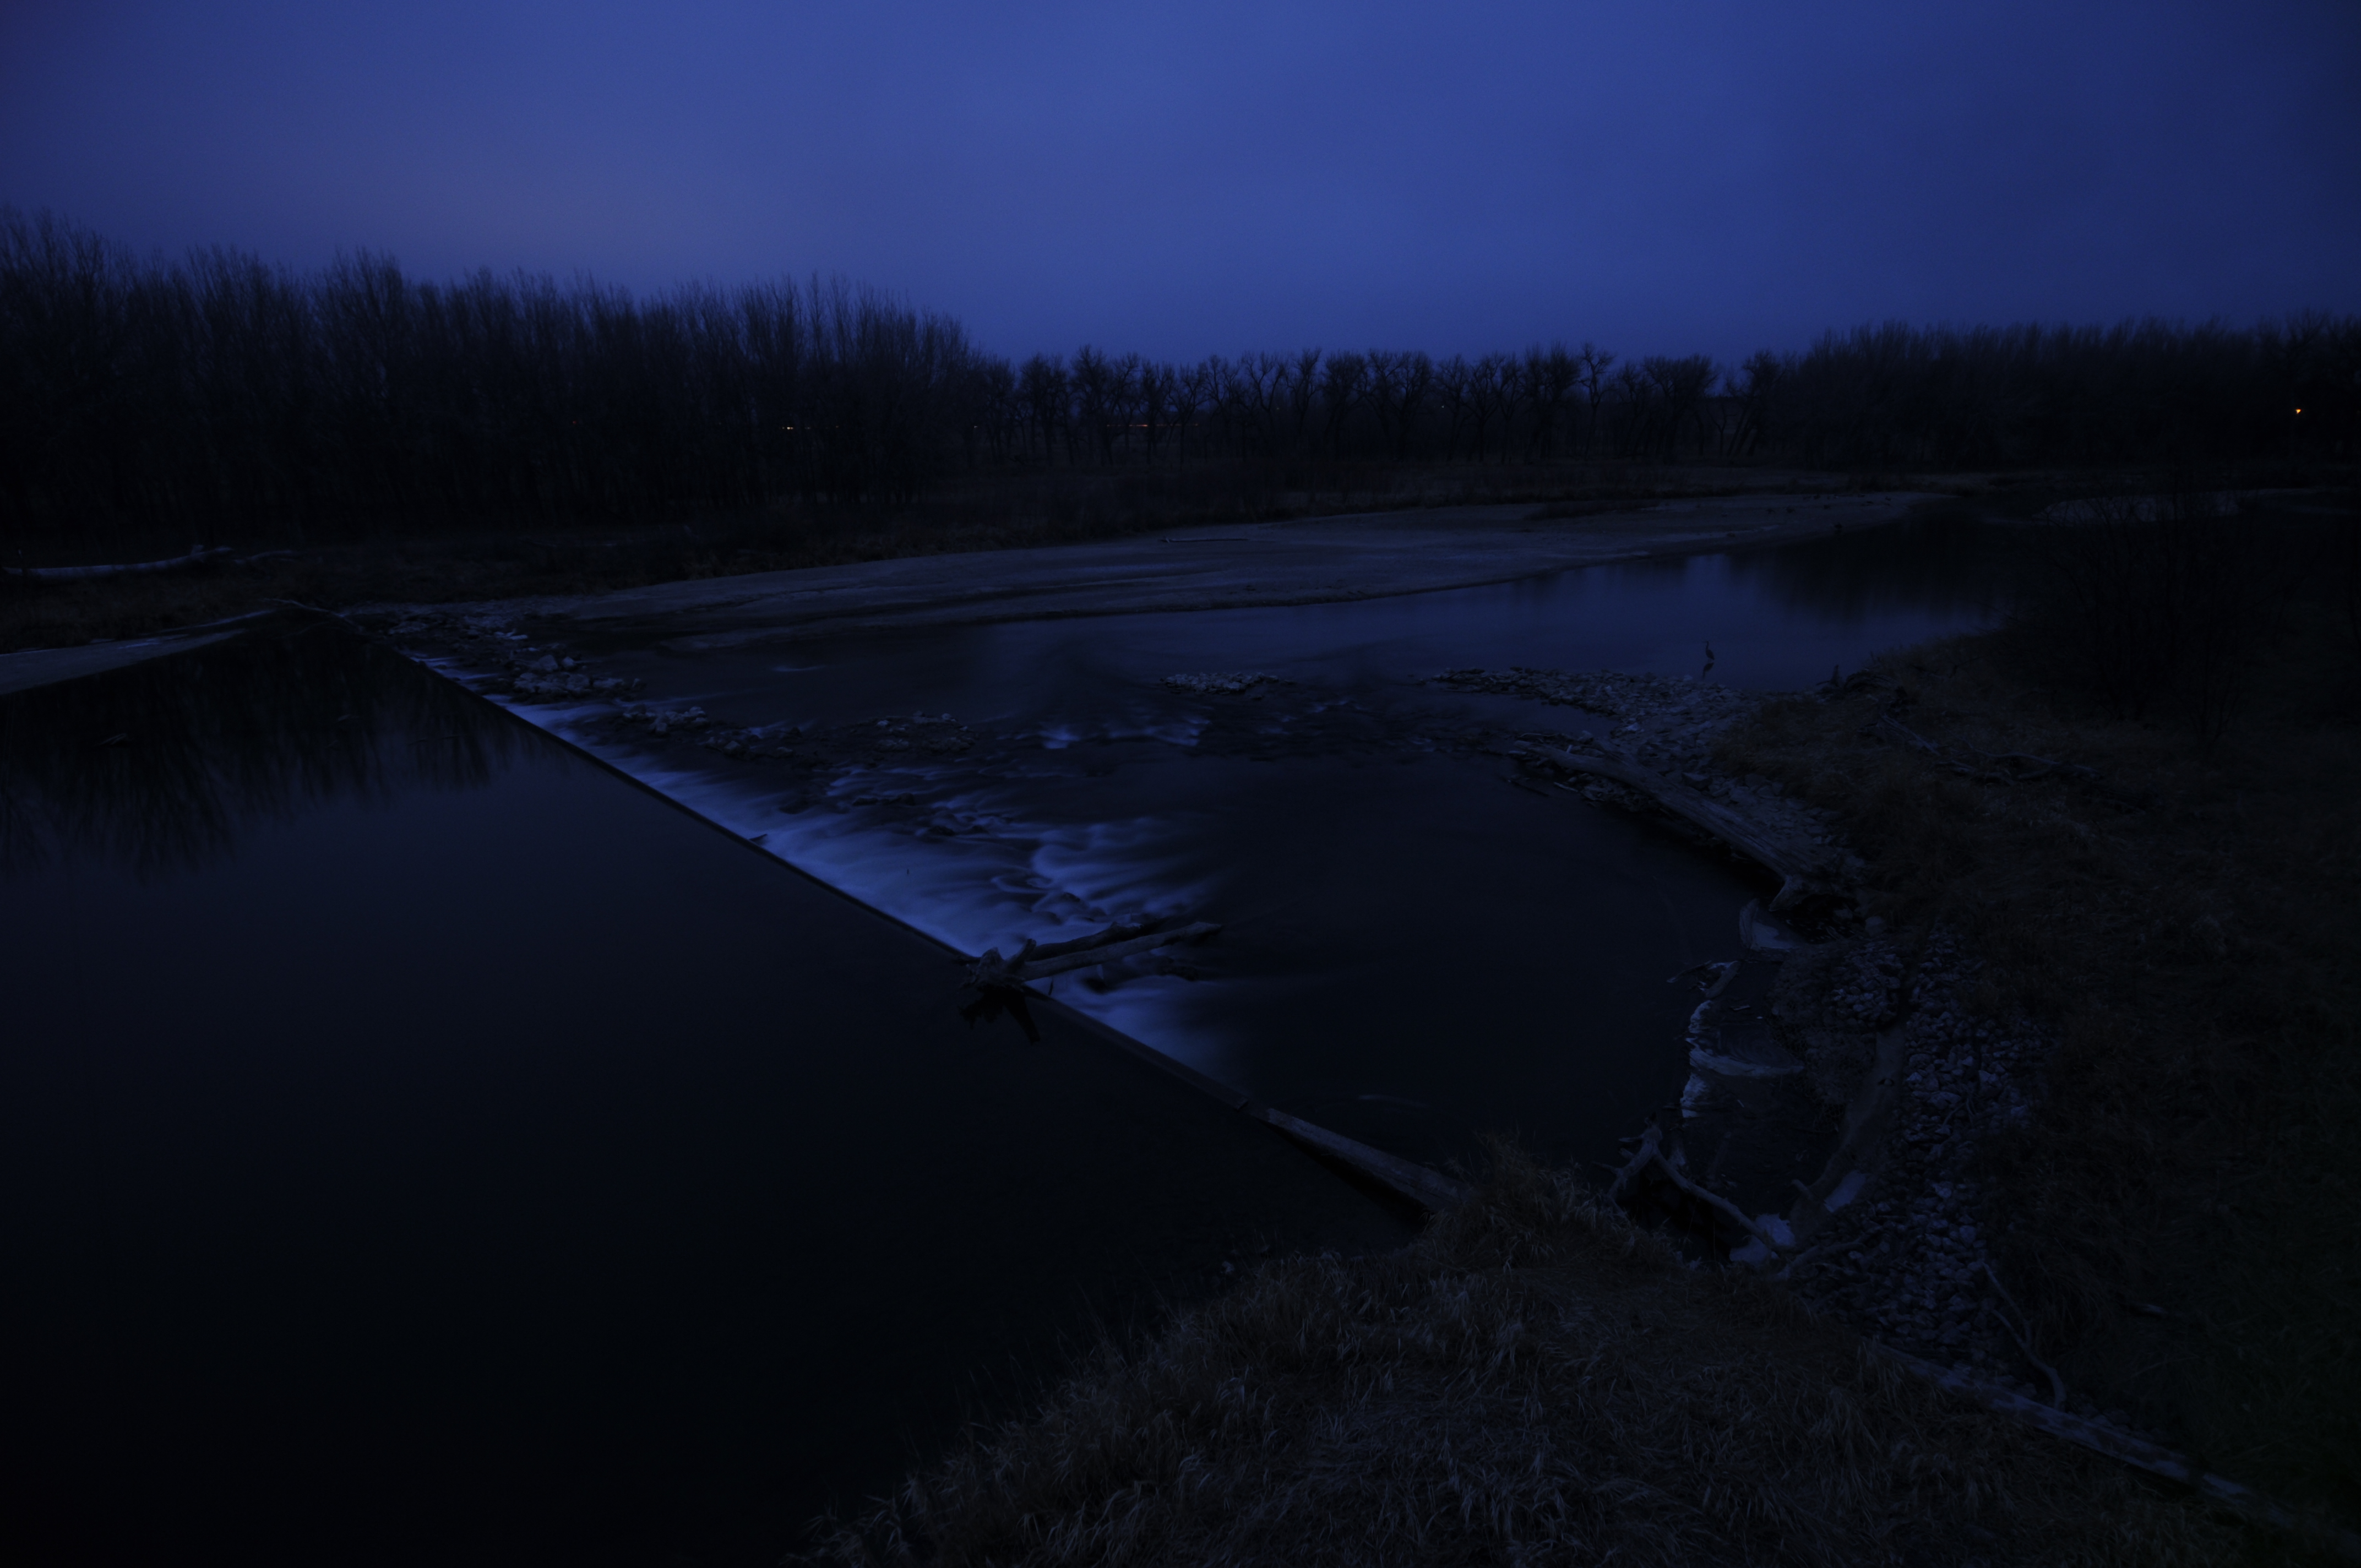
\includegraphics[scale=0.1]{StateLineWeir_20190116_Farrell_805.jpg} 
        \includegraphics[scale=0.1]{StateLineWeir_20190122_Farrell_984.jpg} \\
\end{center}
\begin{center}
        \includegraphics[scale=0.1]{StateLineWeir_20160512_Farrell_061.JPG} 
        \includegraphics[scale=0.1]{StateLineWeir_20151015_Farrell_924.JPG} \\
    \textbf{Ejemplo de cuatro clases de imagenes encontrables (figura 5.0.1)} 
\end{center}

\subsection{Entrenamiento y evaluación del modelo }


Al igual que en la sección anterior del documento, dividimos nuestras imagenes en training, validation y testing, todo esto a la par que importamos las fotografías, también se definió el tamaño inicial y el batch size para el entrenamiento del modelo. La distribución de imágenes fué la siguiente: 

\begin{center}
    \begin{tabular}{|c|c|c|}
    \hline
    group & images & classes  \\
    training & 571 & 2  \\
    testing & 580 & 2  \\
    validation & 571 & 2  \\
    \hline
    \end{tabular}\\
    
    \textbf{Distribución de las imágenes (figura 5.1.1)}
\end{center}







\end{document}
